%-----------------------------------------------------------------------------%
\addChapter{Lampiran 1 : Kuesioner Penelitian}
\chapter*{Lampiran 1 : Kuesioner Penelitian}
%-----------------------------------------------------------------------------%
Responden Yth.\\
Saya \textbf{Aldi Reinaldi}, Mahasiswa Ilmu Komputer angkatan 2011 dari Fakultas Ilmu Komputer Universitas Indonesia. Saat ini saya sedang mengerjakan tugas akhir dengan topik Usability Testing Website Direktorat Jenderal Pajak. Penelitian ini bertujuan untuk membuat dan mengembangkan Prototype User Interface agar dapat membandingkan aspek kegunaan, kenyamanan serta fungsionalitas website direktorat jenderal pajak milik Indonesia dengan India. Sehingga dapat dijadikan masukkan, saran dan kritisi dalam pengembangan website E-Government dalam bidang tersebut.
\newline\\
Oleh karena itu, saya mohon partisipasi anda untuk mengisi kuesioner ini. Seluruh data yang anda berikan hanya digunakan untuk kepentingan penelitian dan akademik.
\newline\\
Salam,\\
Aldi Reinaldi\\
Ilmu Komputer 2011\\
Fakultas Ilmu Komputer $-$ Universitas Indonesia\\
E-mail: arreinaldi@gmail.com | aldi.reinaldi@ui.ac.id

\includepdf[pagecommand={}, pages=2-8]{pics/kuesioner.pdf}
%-----------------------------------------------------------------------------%
\addChapter{Lampiran 2 : Hasil Kuesioner}
%-----------------------------------------------------------------------------%
\begin{landscape}
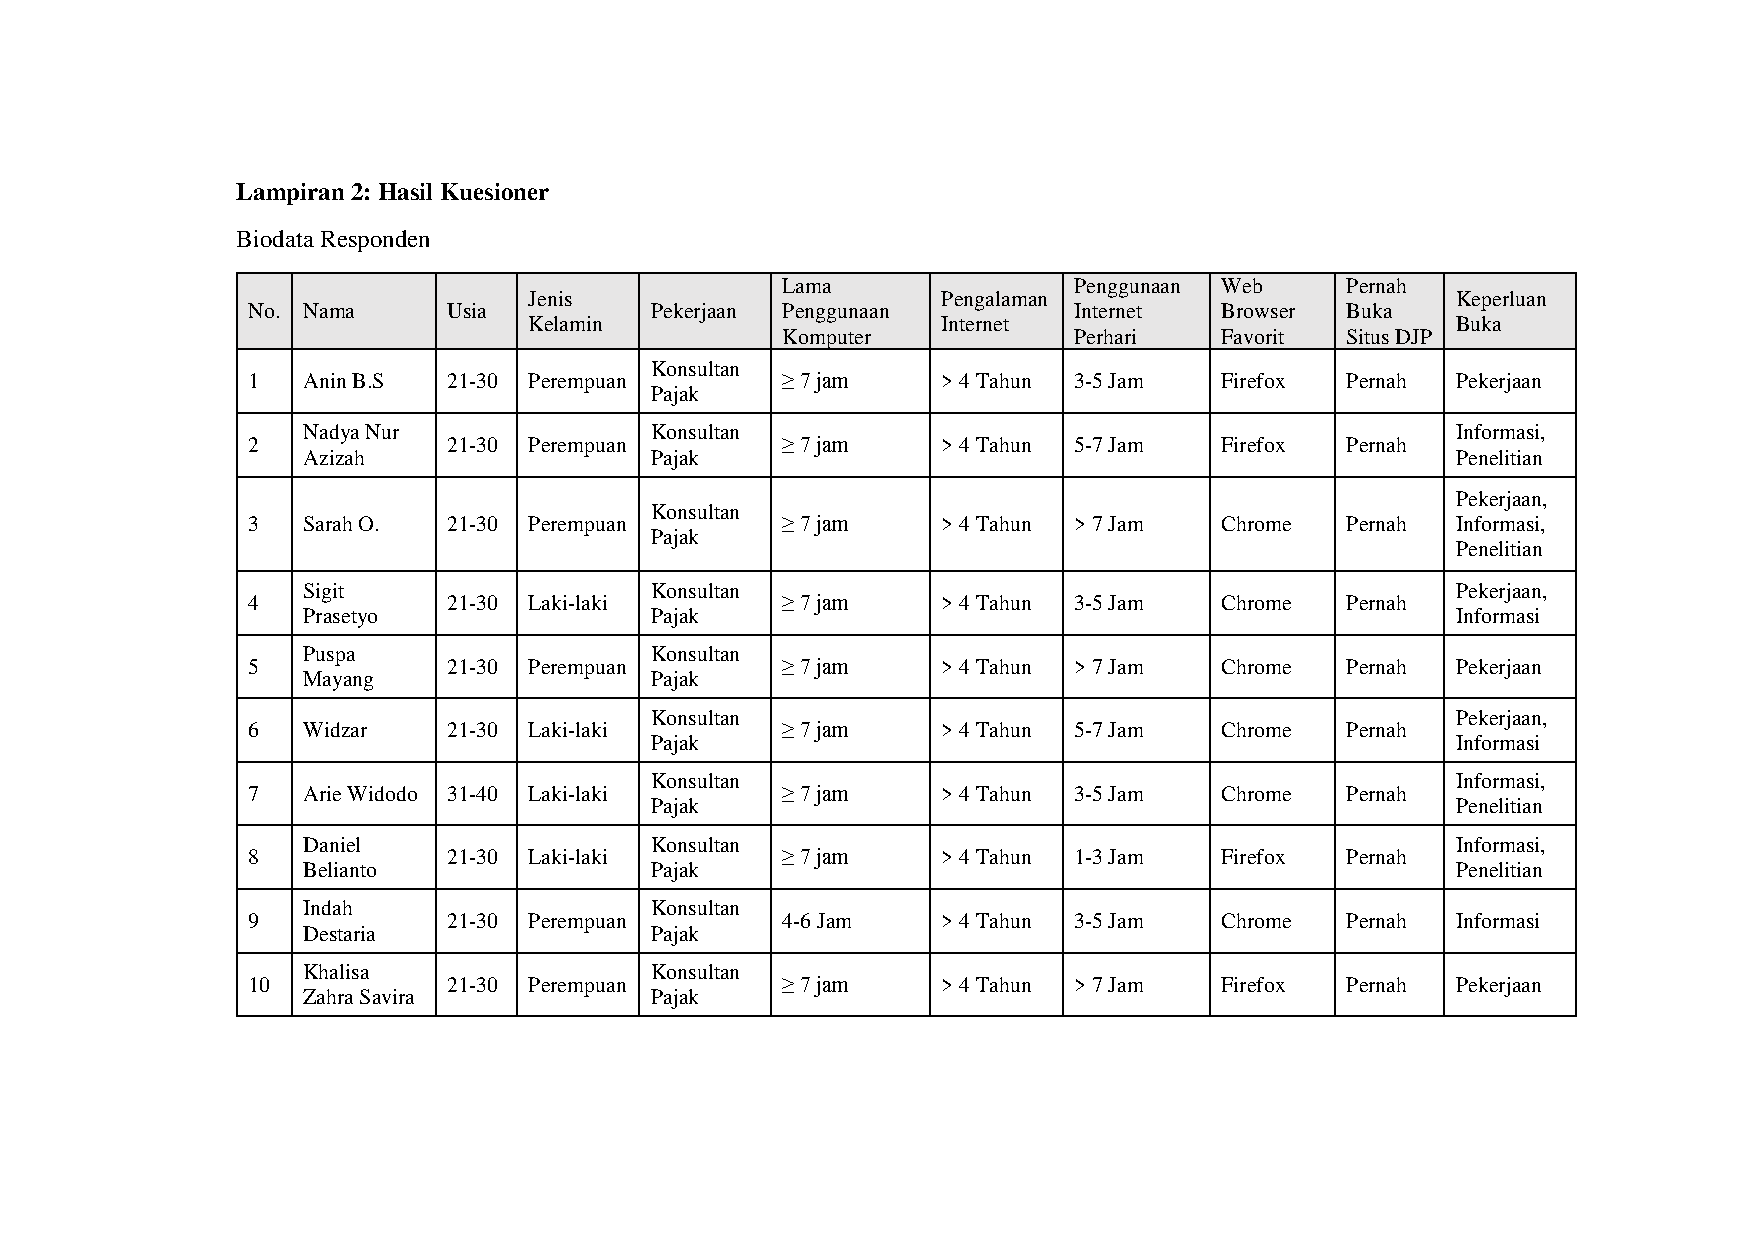
\includepdf[pagecommand={}, pages={-},fitpaper,landscape=true]{pics/rekapdokumen}

\end{landscape}
%-----------------------------------------------------------------------------%
\addChapter{Lampiran 3 : Izin Penelitian DJP}
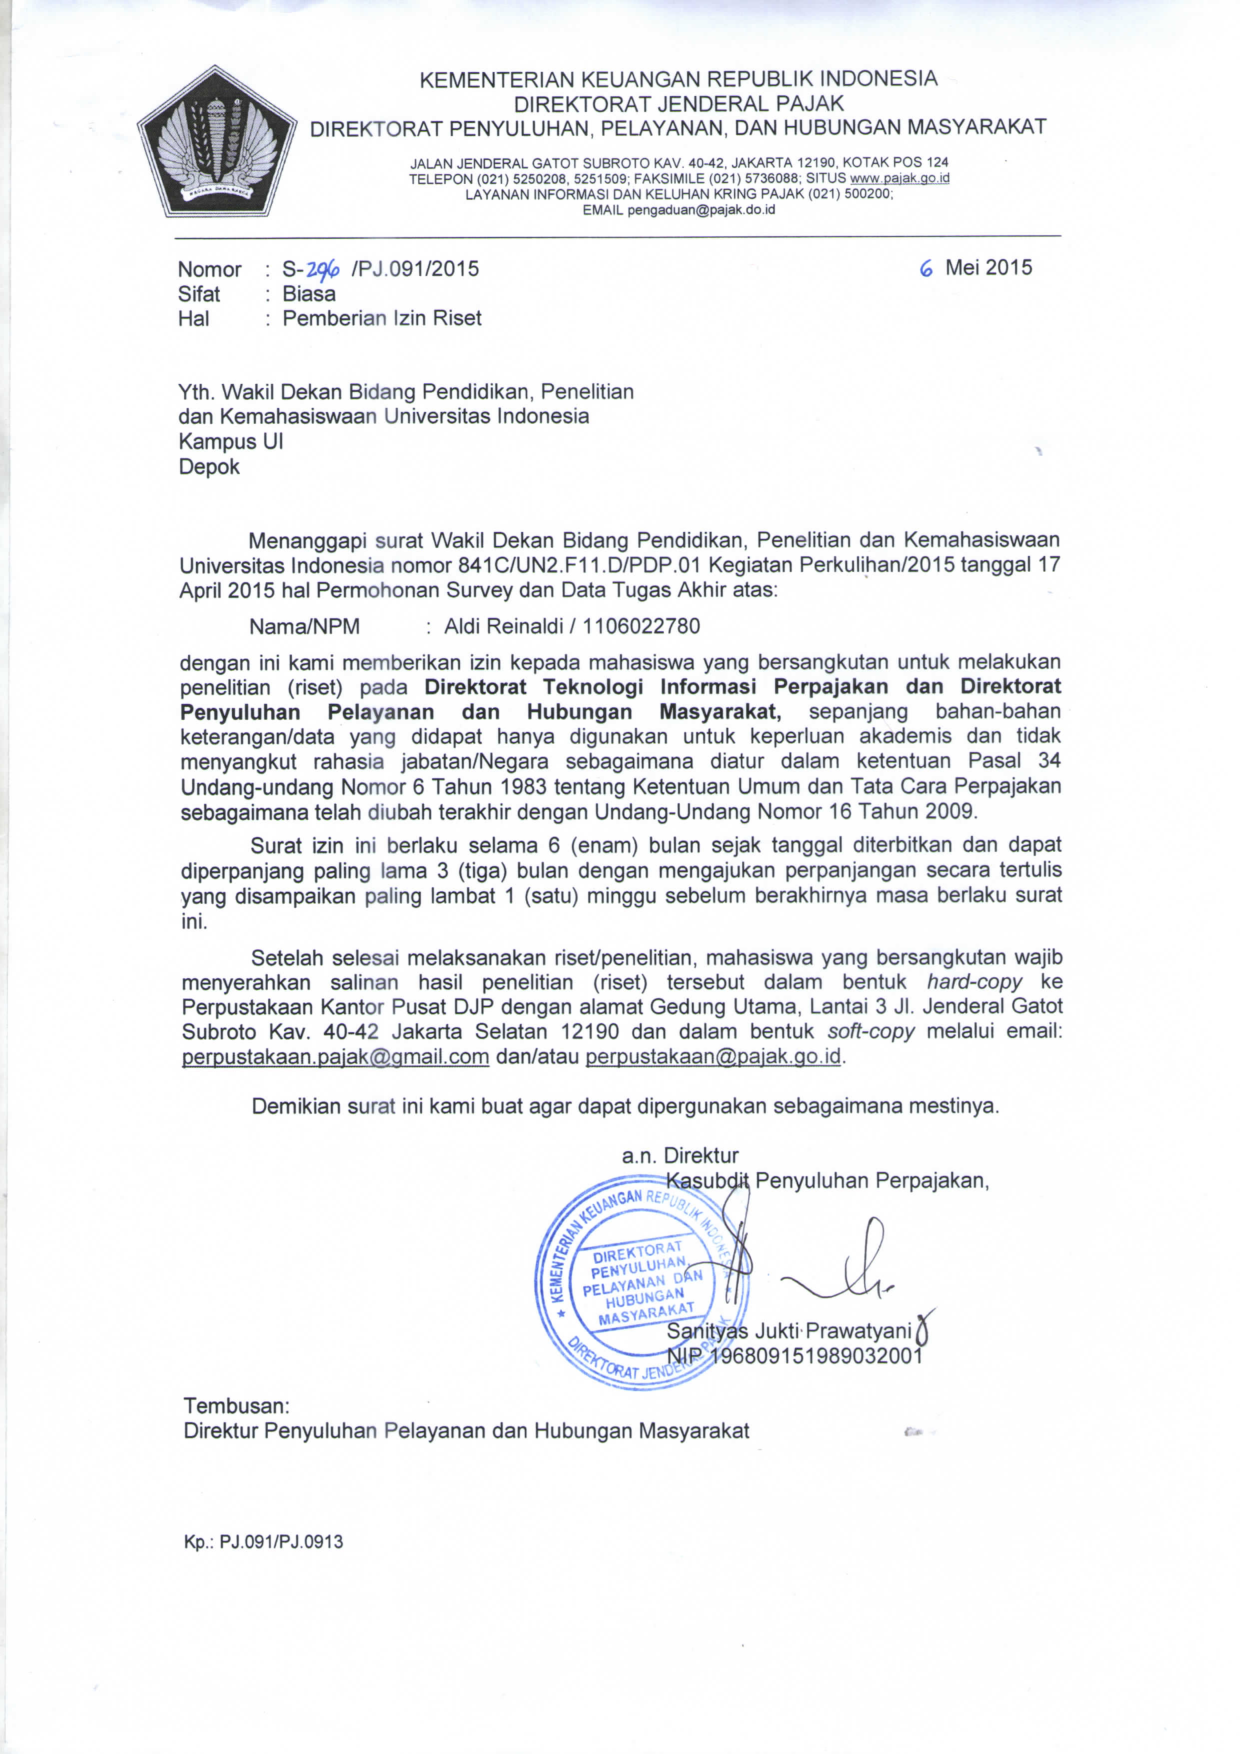
\includepdf[pagecommand={}, pages={-}, fitpaper]{pics/suratdjp.pdf}
%-----------------------------------------------------------------------------%


